\documentclass[11pt,a4paper]{ctexart}

\usepackage[margin=2.6cm]{geometry}
\usepackage{amsmath,amssymb,amsthm}
\usepackage{graphicx}
\usepackage{booktabs}
\usepackage{hyperref}
\usepackage{xcolor}
\usepackage{listings}
\usepackage{caption}

\graphicspath{{figures/}}
\hypersetup{colorlinks=true, linkcolor=blue!50!black, urlcolor=blue!60!black}
\lstset{
  basicstyle=\ttfamily\small,
  breaklines=true,
  frame=single,
  columns=fullflexible,
  backgroundcolor=\color{gray!7}
}

\newtheorem{definition}{定义}[section]
\newtheorem{theorem}{定理}[section]
\newtheorem{lemma}{引理}[section]
\newtheorem{proposition}{命题}[section]
\newtheorem{example}{例}[section]

\title{第 5 章 \quad A review of some results from multivariate analysis / 多元分析结果回顾}
\author{基于 \textit{A Course in Time Series Analysis} 的中文讲义与 Python 实践}
\date{}

\begin{document}
\maketitle

\section*{本章学习目标}

本章按照原文 \textit{A review of some results from multivariate analysis} 的小节顺序整理，保留主要定义、定理、模型公式和练习方向，并将原文中的 R 实践思路改写为 Python 工程实践。

完成本章后，应能够：
\begin{itemize}
  \item 复习内积、范数、正交和投影；
  \item 把线性预测理解为 Hilbert 空间投影；
  \item 推导多阶段投影和偏相关；
  \item 理解精度矩阵中的零元素与条件不相关的关系；
  \item 为后续 Durbin-Levinson 和部分自相关建立几何语言。
\end{itemize}

\section{欧氏空间与投影}

\subsection{内积、范数与正交}

在 \(\mathbb R^n\) 中，内积为
\[
  \langle x,y\rangle=\sum_{i=1}^n x_i y_i,
\]
范数为 \(\|x\|=\sqrt{\langle x,x\rangle}\)。若 \(\langle x,y\rangle=0\)，称 \(x\) 与 \(y\) 正交。

\subsection{投影}

把向量 \(Y\) 投影到由 \(X\) 张成的空间，得到
\[
  \hat Y=\alpha X,\qquad
  \alpha=\frac{\langle Y,X\rangle}{\langle X,X\rangle}.
\]
残差 \(Y-\hat Y\) 与 \(X\) 正交。多元情形中，若 \(X\) 为设计矩阵，则
\[
  \hat Y=X(X'X)^{-1}X'Y.
\]
投影矩阵 \(P=X(X'X)^{-1}X'\) 满足 \(P^2=P\) 和 \(P'=P\)。

\subsection{多阶段投影}

若先投影到一个子空间，再对残差投影到另一个正交补空间，可以把复杂预测分解为几个正交部分。这一思想在后续部分自相关和 Durbin-Levinson 递推中反复出现。

\section{随机变量空间}

二阶随机变量构成一个带内积的空间：
\[
  \langle X,Y\rangle=E(XY).
\]
若使用中心化随机变量，则内积对应协方差：
\[
  \langle X-E X,Y-EY\rangle=\mathrm{cov}(X,Y).
\]
因此，最佳线性预测就是在随机变量空间中的正交投影。

\section{线性预测}

设要用 \(X_1,\ldots,X_p\) 线性预测 \(Y\)，预测量为
\[
  \hat Y=\sum_{j=1}^p a_jX_j.
\]
最优系数由正交方程给出：
\[
  E\left[(Y-\hat Y)X_k\right]=0,\qquad k=1,\ldots,p.
\]
写成矩阵形式：
\[
  \Gamma a=\gamma,
\]
其中 \(\Gamma_{ij}=E(X_iX_j)\)，\(\gamma_i=E(YX_i)\)。

\section{偏相关}

偏相关衡量在控制其他变量后两个变量之间剩余的线性关系。设 \(X\) 与 \(Y\) 都先对 \(Z\) 做线性投影，残差分别为
\[
  X^\perp=X-\mathrm{Proj}(X\mid Z),\qquad
  Y^\perp=Y-\mathrm{Proj}(Y\mid Z).
\]
则偏相关为
\[
  \rho_{XY\cdot Z}
  =\frac{\mathrm{cov}(X^\perp,Y^\perp)}
  {\sqrt{\mathrm{var}(X^\perp)\mathrm{var}(Y^\perp)}}.
\]
在时间序列中，部分自相关就是 \(X_t\) 与 \(X_{t+h}\) 在控制中间 \(X_{t+1},\ldots,X_{t+h-1}\) 后的相关。

\section{精度矩阵性质}

协方差矩阵 \(\Sigma\) 的逆矩阵
\[
  \Omega=\Sigma^{-1}
\]
称为精度矩阵。若随机向量为高斯分布，则 \(\Omega_{ij}=0\) 等价于第 \(i\) 与第 \(j\) 个分量在给定其他分量后条件独立。即使非高斯，精度矩阵的零元素也对应线性条件不相关结构。

\section{附录：Hilbert 空间投影}

原文附录把投影定理放在 Hilbert 空间中陈述：若 \(\mathcal M\) 是闭线性子空间，则任意 \(Y\) 可唯一分解为
\[
  Y=\mathrm{Proj}_{\mathcal M}Y+e,
  \qquad e\perp \mathcal M.
\]
该定理是预测理论的几何基础。

\section{原文例题与定义补充}

\begin{example}[原文 Example 5.3.1：三个随机向量]
原文构造 \(X_1,X_2,X_3\) 三个随机向量，用来说明普通相关和偏相关可能给出不同结论。即使 \(X_1\) 与 \(X_2\) 有相关性，在控制 \(X_3\) 后二者的残差相关也可能消失。
\end{example}

\begin{definition}[原文 Definition 5.5.1：投影]
随机变量 \(Y\) 到由 \(X_1,\ldots,X_p\) 张成空间的投影，是该空间中使均方误差
\[
  E(Y-\hat Y)^2
\]
最小的元素 \(\hat Y\)。残差 \(Y-\hat Y\) 与所有解释变量正交。
\end{definition}

\begin{example}[原文 Example 5.5.1：Hilbert 空间]
\(\mathbb R^n\) 是有限维 Hilbert 空间；二阶随机变量在内积 \(E(XY)\) 下也形成 Hilbert 空间。预测理论把这两个例子统一起来。
\end{example}

第 5.4 节的证明说明，精度矩阵零元素与残差正交关系等价；第 5.5 节附录则把欧氏投影推广到闭线性子空间，为后续时间序列预测提供抽象框架。

\section{Python 工程实践}

在本章目录下运行：
\begin{lstlisting}[language=bash]
python scripts/ch05_generate_figures.py
\end{lstlisting}

脚本会把图像写入本章 \texttt{figures/} 目录。当前图像用于配合本章核心概念的仿真说明；若后续补齐原始数据文件，可把模拟数据替换为原文真实数据案例。

\begin{figure}[htbp]
  \centering
  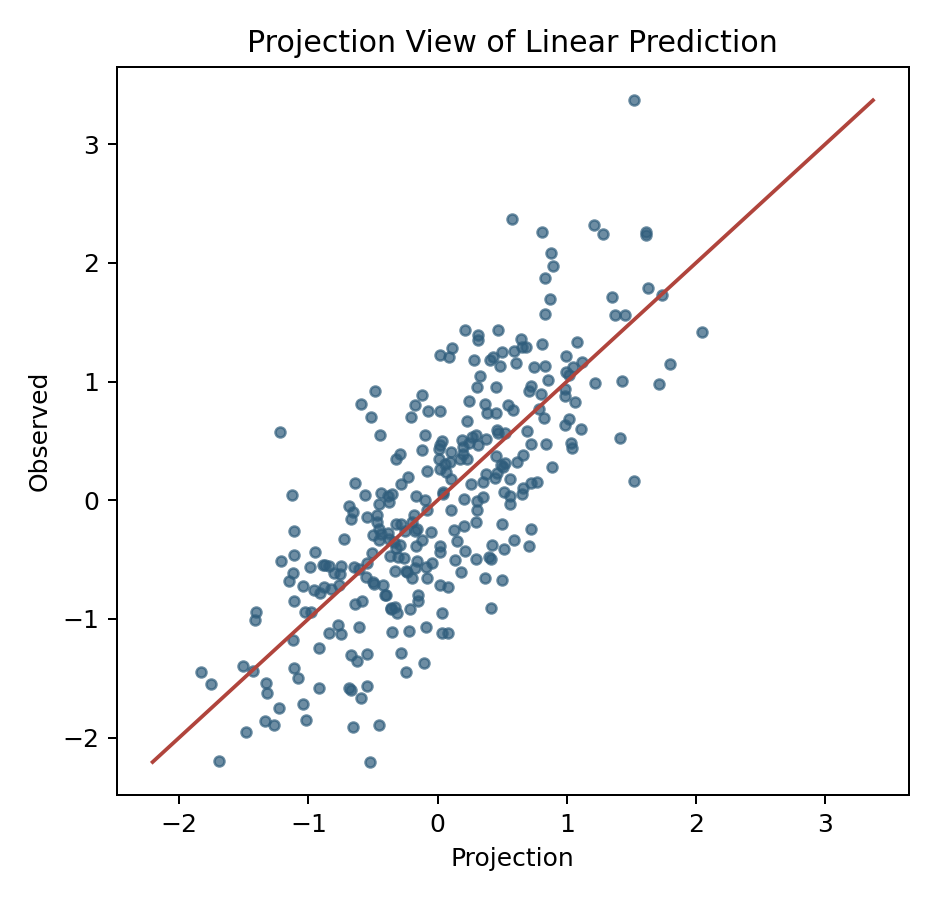
\includegraphics[width=0.86\textwidth]{ch05_fig01_projection_prediction.png}
  \caption{线性预测的投影视角：预测值是观测向解释变量空间的正交投影。}
\end{figure}

\begin{figure}[htbp]
  \centering
  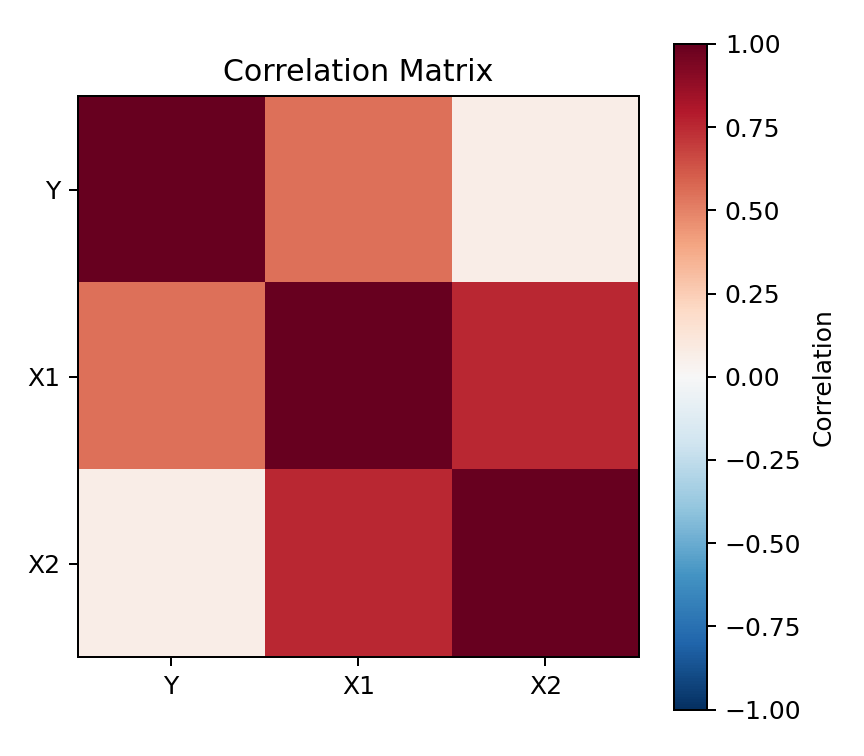
\includegraphics[width=0.86\textwidth]{ch05_fig02_correlation_matrix.png}
  \caption{相关矩阵示例：多元关系可由协方差矩阵和精度矩阵进一步分析。}
\end{figure}

\section{练习提要}

原文练习主要围绕下列方向展开：
\begin{itemize}
  \item 计算向量投影和投影残差，验证正交性；
  \item 推导最优线性预测的正规方程；
  \item 用残差相关解释偏相关；
  \item 从协方差矩阵求精度矩阵并解释零元素。
\end{itemize}

\section*{本章小结}

第 5 章把多元线性代数翻译成时间序列预测语言。投影给出最小均方误差预测，偏相关解释 PACF，精度矩阵则连接到条件依赖结构。

\end{document}
